\section{Aprendizaje Automático}

\begin{frame}
    \frametitle{Aprendizaje Automático}

    \begin{itemize}
        \item Objetivo: hacer aprender a una computadora
        \item En la \emph{clasificación} se intenta aprender la categoría de una entidad.
    \end{itemize}
\end{frame}

\subsection{Clasificadores}
\begin{frame}
    \frametitle{Clasificadores}
    
    \begin{itemize}
        \item Un clasificador decide en base a \emph{características} y a ciertas suposiciones.
    \end{itemize}
\end{frame}

\subsection{Metodología}
\begin{frame}
    \frametitle{Metodología}

    \begin{itemize}
        \item Entrenamiento y evaluación
    \end{itemize}
\end{frame}
\note{
    TODO: explicar qué es Entrenamiento y qué es Evaluación.
}

\begin{frame}
    \frametitle{Support Vector Machine (SVM)}

    \begin{center}
        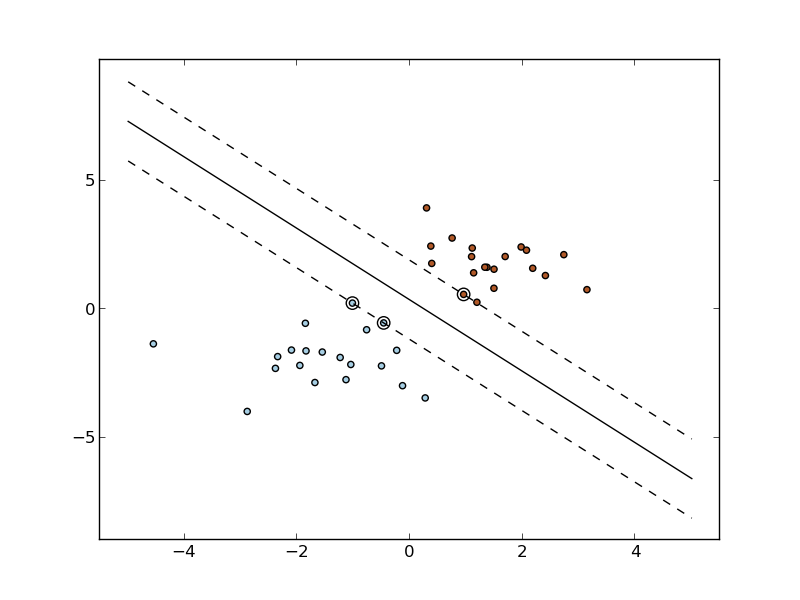
\includegraphics{svm.png}
    \end{center}
\end{frame}

\begin{frame}
    \frametitle{Árbol de decisión (DT)}

    \begin{center}
        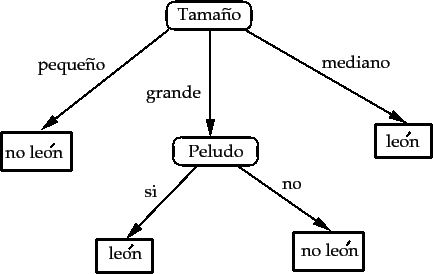
\includegraphics{dts.png}
    \end{center}
\end{frame}

\begin{frame}
    \frametitle{Naïve Bayes (NB)}

    \begin{center}
        \[
            P(A|B) = \frac{P(B|A) P(A)}{P(B)}
        \]

        \begin{align*}
            c &= \argmax_{c \in C} P(c|a_1, \ldots, a_n) \\
            &= \argmax_{c \in C} \frac{P(a_1, \ldots, a_n|c) P(c)}{P(a_1, \ldots, a_n)} \\
            &= \argmax_{c \in C} P(a_1, \ldots, a_n|c) P(c) \\
            &\approx \argmax_{c \in C} P(c) \prod_{i=1}^n P(a_i|c) \\
        \end{align*}
    \end{center}
\end{frame}

\begin{frame}
    \frametitle{k Nearest Neighbors (kNN)}

    \begin{center}
        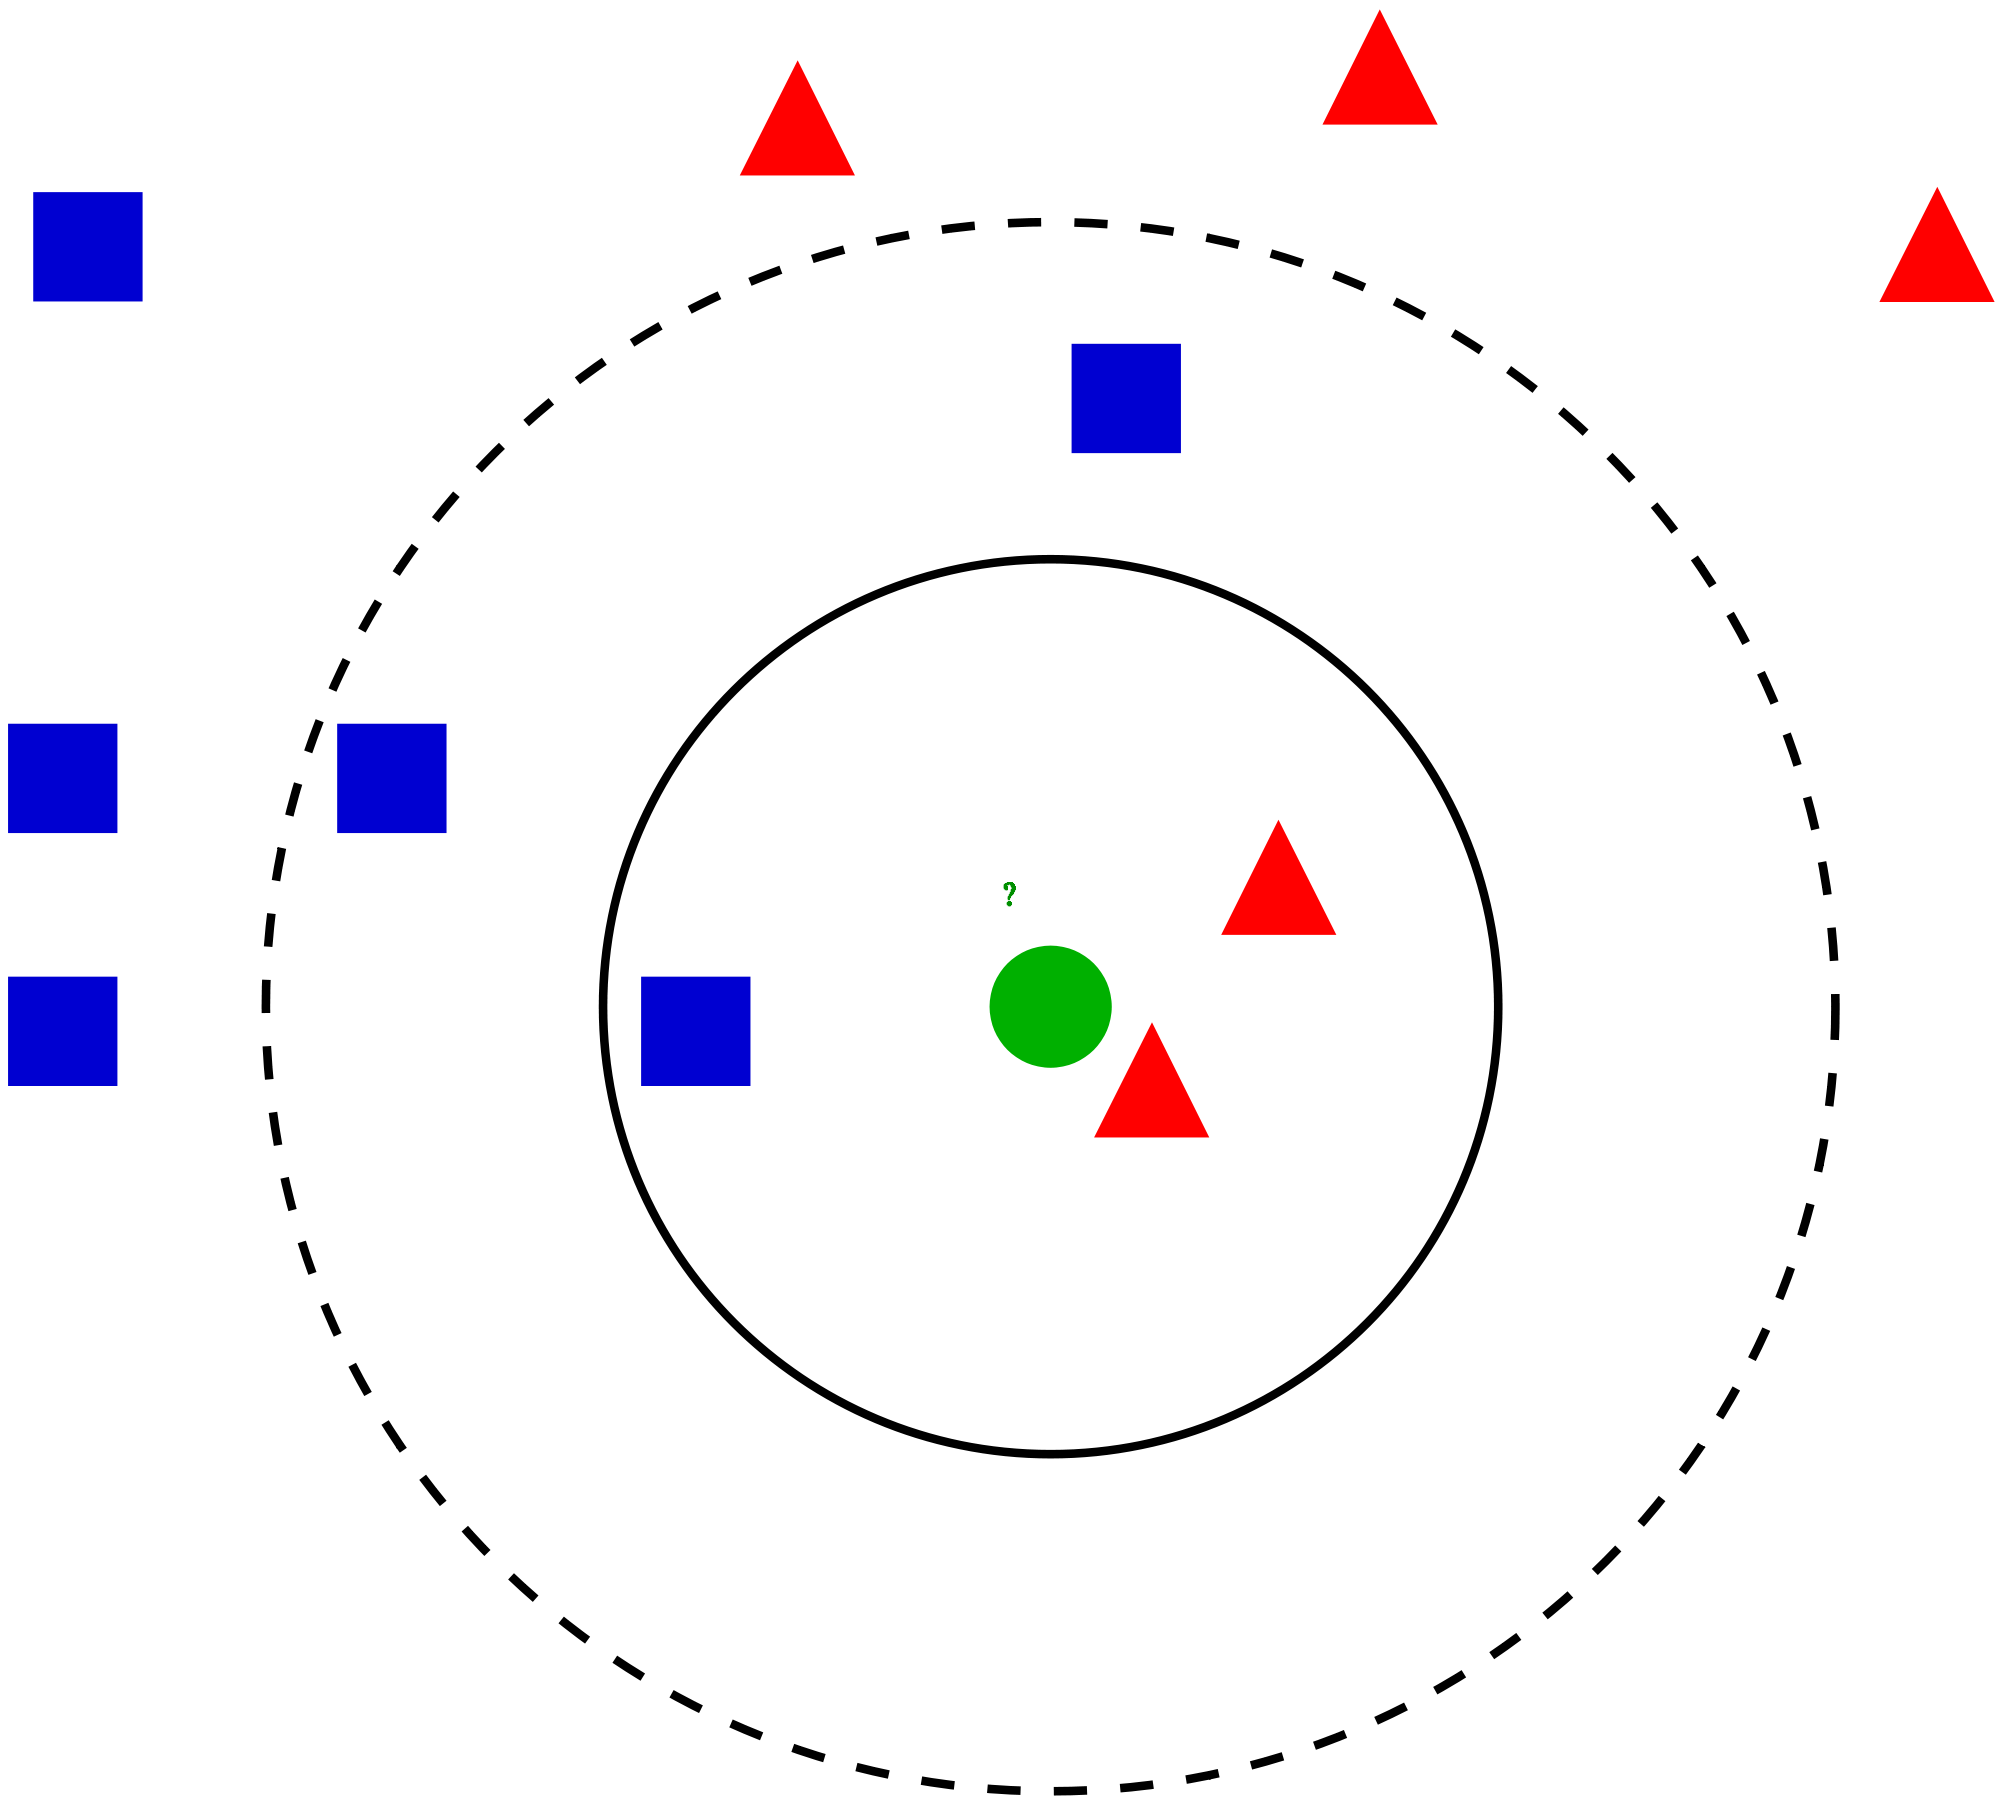
\includegraphics{knn.png}
    \end{center}
\end{frame}
\note{\textbf{k Nearest Neighbors} (kNN), o los \emph{k} vecinos más cercanos, es un tipo de clasificador que para predecir el valor de una instancia mira otras consideradas cercanas. De manera similar a SVM usa un espacio vectorial para representar las instancias. El dibujo ilustra que se quiere clasificar el círculo como rojo o azul. Mirando las tres más cercanas, se da por rojo, aunque las cinco más cercanas da por ejemplo azul. El \emph{k} influye. También se puede hacer ponderar la distancia de las instancias más cercanas.}

\subsection{Métricas}
\begin{frame}
    \frametitle{Métricas}
    
    \begin{columns}[T]
        \begin{column}[T]{.4\textwidth}
            \begin{block}{Tipos de instancias}
                \begin{itemize}
                    \item Verdaderos positivos
                    \item Falsos positivos
                    \item Falsos negativos
                    \item Verdaderos negativos
                \end{itemize}
            \end{block}

            \begin{block}{Medidas}
                \begin{itemize}
                    \item Precisión, $P = \frac{VP}{VP + FP}$
                    \item Recall, $R = \frac{VP}{VP + FN}$
                    \item $F_1 = \frac{2 P R}{P + R} = \frac{VP}{VP + \frac{FP + FN}{2}}$
                    \item Acierto $= \frac{VP + VN}{VP + VN + FP + FN}$
                \end{itemize}
            \end{block}
        \end{column}

        \begin{column}[T]{.6\textwidth}
            \begin{center}
                \includesvg[height=7cm, svgpath=imagenes/]{medidas}
            \end{center}
        \end{column}
    \end{columns}
\end{frame}
\note{
    Es importante contar con medidas para poder evaluar el desempeño de un aprendiz y poder compararlo con otros.

    En el caso de la clasificación es necesario distinguir a las instancias según el tipo de resultado obtenido. La imagen puede ayudar a identificarlos. La primera es \textbf{Verdaderos positivos}, que es la parte verde dentro de la elipse. En la imagen yo quiero distinguir los puntos rellenos, y esta clase son aquellos que clasifiqué correctamente de los rellenos. Los \textbf{Falsos positivos} son los que clasifiqué incorrectamente, es decir la parte roja de la elipse. En la elipse están todos los que yo dije que eran positivos. Luego los \textbf{Falsos negativos} son la parte roja fuera de la elipse, que el clasificador dijo que eran negativos pero en realidad son puntos rellenos, por lo tanto ``no los encontré''. Luego están los \textbf{Verdaderos negativos} que son aquellos que correctamente dejé afuera, y es la partición que queda de la ilustración.
}
\note{
    A partir de lo anterior, se definen 4 medidas. \textbf{Precisión} (ilustrada por la P en el dibujo) es el porcentaje de instancias correctamente etiquetadas como positivas. Es la relación entre la parte verde de la elipse y la elipse en sí (no le importan los negativos). Presta atención a los errores de tipo I (falsos positivos). El \textbf{Recall} (ilustrado por la R en el dibujo) mide la relación entre los correctamente encontrados respecto a todos los que positivos había. De esta manera presta atención a los errores de tipo II (falsos negativos). Tampoco le importa la correcta clasificación de los negativos. La medida \textbf{$F_1$} es muy similar a las anteriores, pero pondera de igual manera los dos tipos de errores. Se puede ver como una medida promedio. A su vez está el \textbf{Acierto}, que es el porcentaje de instancias correctamente clasificadas (de cualquier tipo, esta sí mira los negativos).
}

\note{
    TODO: resumir esto y hablar en la parte de resultados.
    
    En algunos tipos de clasificadores, como SVM y kNN, hay una función de distancia implícitamente definida, en la cual los distintos valores de cada característica imponen un peso en la misma. Por ejemplo, si se tiene una característica binaria que indica con 0 o 1 la presencia de cierta palabra en un tweet y otra característica que cuenta la cantidad de letras, la última toma valores muchos más grandes y una diferencia de dos letras en un tweet representarían una distancia mayor que dos tweets con distintos valores en la primera característica, aunque no necesariamente es cierto que una distancia sea mayor que la otra. A métodos que estandaricen los datos de esta manera se dice que hacen Escalado de características. Se puede resolver este problema realizando un Reescalado, dejando los valores de todas las características en el mismo rango, como [0, 1], por ejemplo. Pero adicionalmente, cuando se entrena con SVM con ciertos tipos de curvas, se asumen que los datos tienen la misma varianza y están centrados en cero. Entonces se preprocesan los valores de los atributos para que queden con promedio cero y desviación estándar uno. A esto se le conoce como Estandarización. Para el caso puntual de MNB no tiene sentido hacer escalado ya que supone que las características tienen distribución multinomial, es decir de un dominio discreto. A su vez el clasificador no permite valores negativos de características, por lo tanto un centrado tampoco aplica.
}
